\documentclass[11pt]{standalone}
\usepackage{amssymb}
\usepackage{amsmath}
\usepackage[no-math]{fontspec}
\usepackage{unicode-math}
\usepackage{libertinus}
\usepackage{pgf,xcolor}
\usepackage{tikz}
\usetikzlibrary{arrows.meta, backgrounds}
\usepackage{pgfplots}
\pgfplotsset{compat=newest}

\definecolor{my_darkgray}{HTML}{484949}
\definecolor{my_lightgray}{HTML}{F3F4F4}
\definecolor{my_darkblue}{HTML}{005A94}
\definecolor{my_lightblue}{HTML}{CCDEE9}
\definecolor{my_yellow}{HTML}{FFEC7F}
\definecolor{my_red}{HTML}{E60000}
\definecolor{my_orange}{HTML}{E87846}

\begin{document}
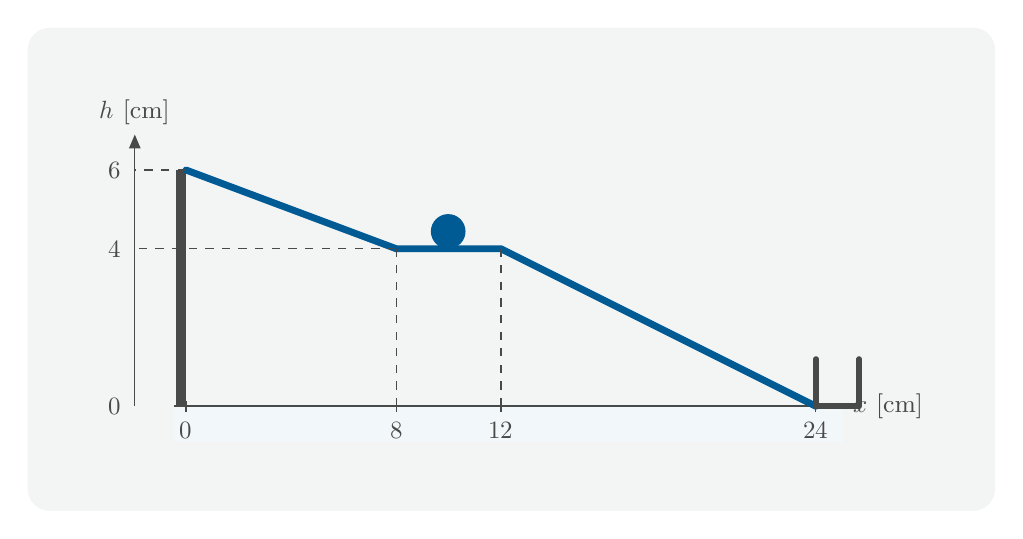
\begin{tikzpicture}[
    show background rectangle,
    background rectangle/.style={fill=my_lightgray, rounded corners=8pt},
    inner frame sep=0.8cm
]

% Coordinate scale: x_draw = x_real / 3,   y_draw = h_real / 2
% Track vertices (x_draw, y_draw):
%   (0,    3.0)  <--  x=0  cm,  h=6 cm  (start)
%   (2.67, 2.0)  <--  x=8  cm,  h=4 cm  (end of segment 1)
%   (4.0,  2.0)  <--  x=12 cm,  h=4 cm  (end of plateau)
%   (8.0,  0.0)  <--  x=24 cm,  h=0 cm  (finish)

% Table surface
\fill[my_lightblue!25] (-0.15,-0.45) rectangle (8.35,0);
\draw[thick, my_darkgray] (-0.15,0) -- (8.35,0);

% Starting block (vertical support at x=0)
\fill[my_darkgray] (-0.13,0) rectangle (0,3.0);

% Track: three segments drawn as one connected path
\draw[my_darkblue, line width=2.5pt, line cap=round, line join=round]
    (0,3.0) -- (2.67,2.0) -- (4.0,2.0) -- (8.0,0.0);

% Finishing block (open catch container at x=24)
\draw[my_darkgray, line width=2pt, line cap=round, line join=round]
    (8.0,0.6) -- (8.0,0) -- (8.55,0) -- (8.55,0.6);

% Marble resting on the plateau (x_real=10, x_draw=3.33, sits on top of track)
\fill[my_darkblue] (3.33,2.22) circle (0.22);

% Dashed vertical lines dropping from segment boundaries to table surface
\draw[dashed, my_darkgray, thin] (2.67,0) -- (2.67,2.0);
\draw[dashed, my_darkgray, thin] (4.0, 0) -- (4.0, 2.0);

% Height annotation axis (left of figure)
\draw[-{Triangle[length=5pt]}, my_darkgray, thin] (-0.65,0) -- (-0.65,3.45);
\node[above, my_darkgray, font=\small] at (-0.65,3.45) {$h$ [cm]};

% Dashed horizontal lines from track heights to annotation axis
\draw[dashed, my_darkgray, thin] (0,    3.0) -- (-0.65, 3.0);
\draw[dashed, my_darkgray, thin] (2.67, 2.0) -- (-0.65, 2.0);

% Height tick labels
\node[left, my_darkgray, font=\small] at (-0.7, 3.0) {$6$};
\node[left, my_darkgray, font=\small] at (-0.7, 2.0) {$4$};
\node[left, my_darkgray, font=\small] at (-0.7, 0.0) {$0$};

% x-axis ticks and labels below the table surface
\foreach \xd/\xl in {0/0, 2.67/8, 4.0/12, 8.0/24} {
    \draw[my_darkgray, thin] (\xd,-0.07) -- (\xd,0.07);
    \node[below, my_darkgray, font=\small] at (\xd,-0.07) {$\xl$};
}
\node[right, my_darkgray, font=\small] at (8.35,0) {$x$ [cm]};

\end{tikzpicture}
\end{document}
